% !TeX spellcheck = es_ANY
\chapter{Fabricación y Resultados}\label{ch:resultados}
\section{Primer modelo}
Tres modelos distintos fueron propuestos para la fabricación del stage. El primero hace uso del sistema de lectura propio de los discos compactos, tales como el CD, DVD y Blu-Ray. Este sistema cuenta con movimiento en dos direcciones, propios de coordenadas cilíndricas. El movimiento en $\theta$ relacionado con traslación en el plano y en $z$ para realizar el enfoque sobre la muestra. 

Usando dos sistemas como el descrito anteriormente y condicionando el experimento a ángulos pequeños es posible obtener un stage aproximado con movimiento $x$, $y$ y $z$.
\begin{equation}
	\begin{matrix}
		x = r\cos\theta \approx r\left(1 - \dfrac{1}{2}\theta^2\right) \\
		y = r\sin\theta \approx r\theta
	\end{matrix}
	\qquad
	\text{donde $r \approx 90$ mm}
\end{equation}

\begin{figure}[h]
	\centering
	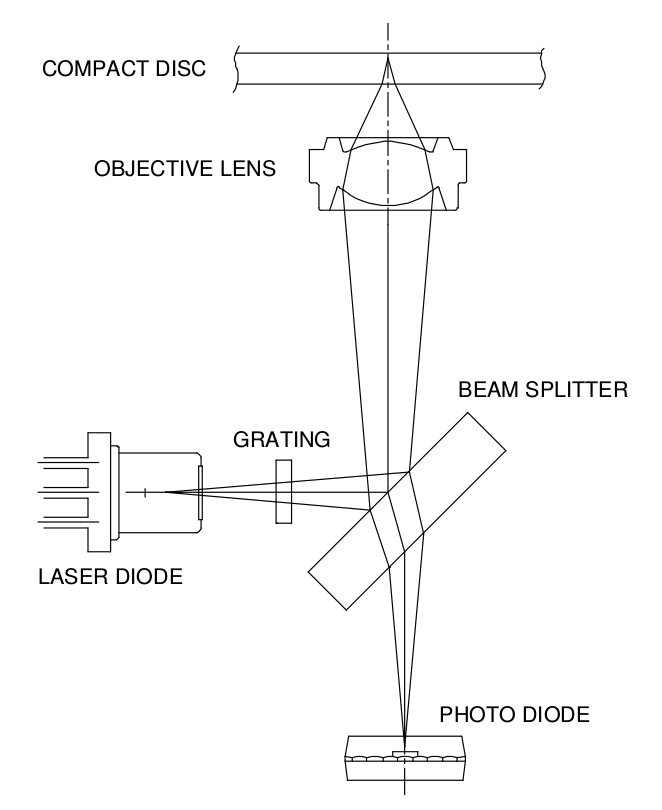
\includegraphics[width=0.3\linewidth]{figures/cdsystem.png}
	\caption{Sistema de detección implementado por la primera versión del stage, el cual hace uso del sistema de lectura de un CD.}
	\label{fig:cdsystem}
\end{figure}

Según el fabricante la distancia máxima de movimiento sobre el plano es de $\pm 0.5$ mm, dando en total $1.0$ mm para translación. En el eje $z$ la distancia máxima es de $\pm$ 0.7 mm, para un total de $1.4$ mm, sin embargo la sensibilidad es de sólo el 20 \%. Usando este stage y aprovechando el interior de los sistemas de lectura de DVDs, se realizó esquema de detección por reflexión, análogo a un microscopio confocal salvo que no existen pinholes el cual se muestra en la \autoref{fig:cdsystem}.

\begin{figure}[h]
	\centering
	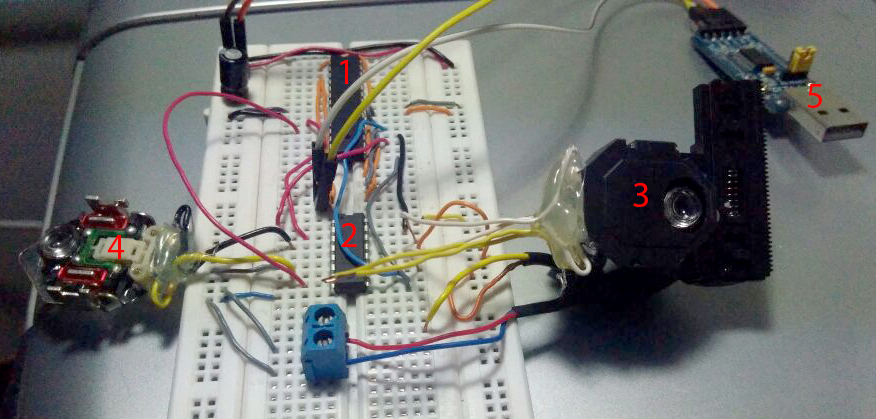
\includegraphics[width=0.8\linewidth]{figures/breadboard}
	\caption{Circuito implementado para el primer stage con etapa de detección. (1) Microcontrolador (Atmega328). (2) Puente H, etapa de potencia para los motores. (3) Sistema \'optico principal con laser y movimiento en $x$. (4) Sistema \'optico con movimiento en $y$. (5) Comunicaci\'on UART.}
	\label{fig:firstsystem}
\end{figure}

El sistema se muestra en la \autoref{fig:firstsystem}. Posicionando el elemento 3 sobre el 4 usando como ayuda una prensa, a la altura donde más pequeño se observó el punto del láser fue posible obtener la imagen que se muestra en la \autoref{fig:firstresults}.

\begin{figure}[h]
	\centering
	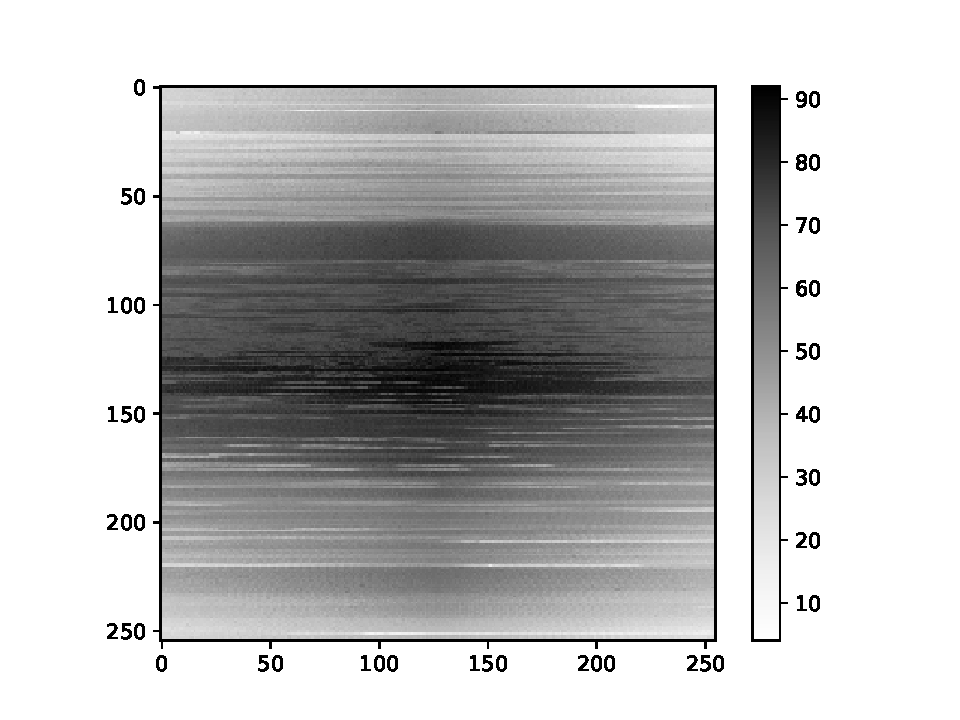
\includegraphics[width=0.62\linewidth]{figures/complete.pdf}
	\caption{Resultados obtenidos usando el primer stage. Se observa la primera línea horizontal de la letra E impresa sobre papel.}
	\label{fig:firstresults}
\end{figure}

El papel con la letra fue tomado de una factura, y se dispuso en la parte superior del lente que se observa en 4, sin ningún tipo de adhesión. De la imagen es importante resaltar que el sistema de detección implementado no cuenta con algún tipo de amplificación, ni de resta del fondo, por lo cual no es posible usar la totalidad de los 10 bits disponibles para la conversión de la señal análoga a digital, y se obtiene únicamente un rango de 0 a 90 valores distintos, lo cual corresponde a 7 bits. Además las condiciones de iluminación del cuarto pudieron alterar los resultados de la medición. En este sentido de implementar un nuevo sistema en el futuro es necesario considerar un sistema de resta en la señal y posterior amplificación de la misma.

Posteriormente y con el objetivo de brindar apoyo en otro proyecto además de simplificar el posicionamiento de la muestra, fueron propuestos dos modelos alternativos.

\section{Segundo modelo}
El segundo modelo propuesto carece de movimiento en la dirección $z$, sin embargo permite un aislamiento del ruido de los motores dado que los mismos se encuentran alejados de la muestra. El movimiento es entonces obtenido al conectar el sistema con los motores usando correas de transporte, los motores serían de paso, conectados al motoreductor que se encuentra a la derecha en la \autoref{fig:secondsystem}, con el objetivo de reducir el tamaño del paso de cada uno de ellos.
\begin{figure}[h]
	\centering
	\begin{tabular}{cc}
		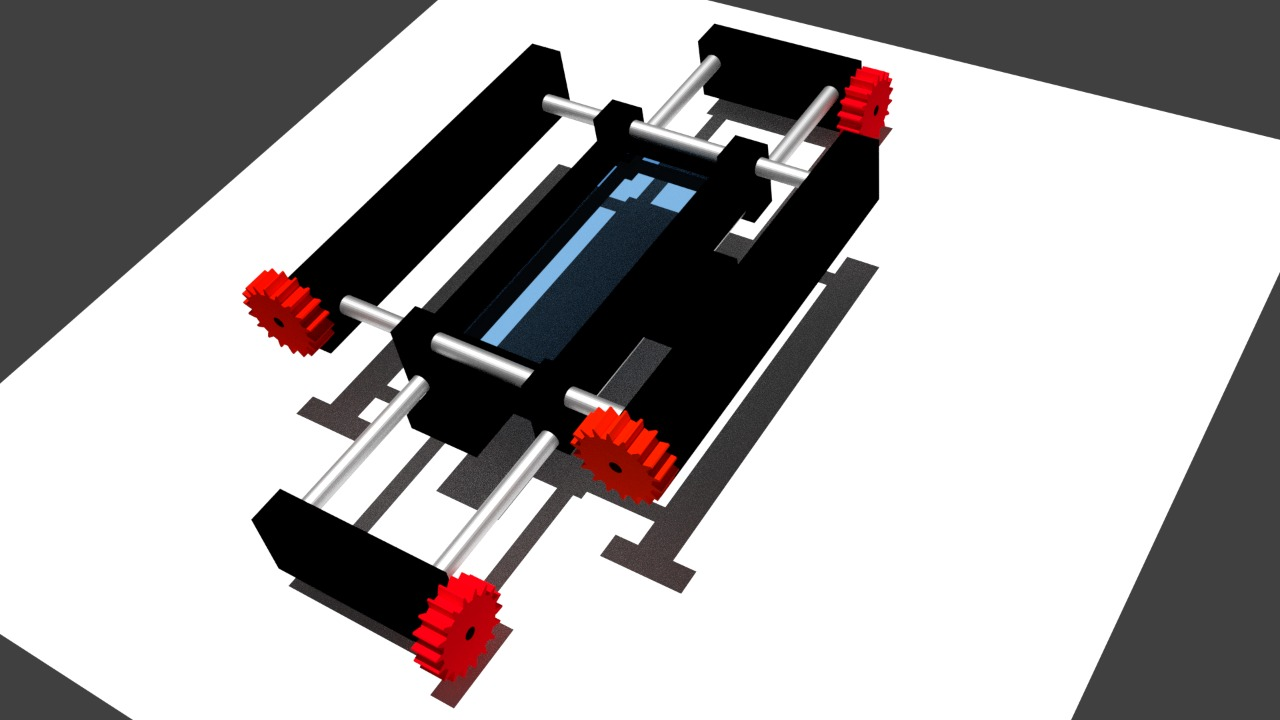
\includegraphics[width=0.45\linewidth]{figures/system2.jpg} & 
		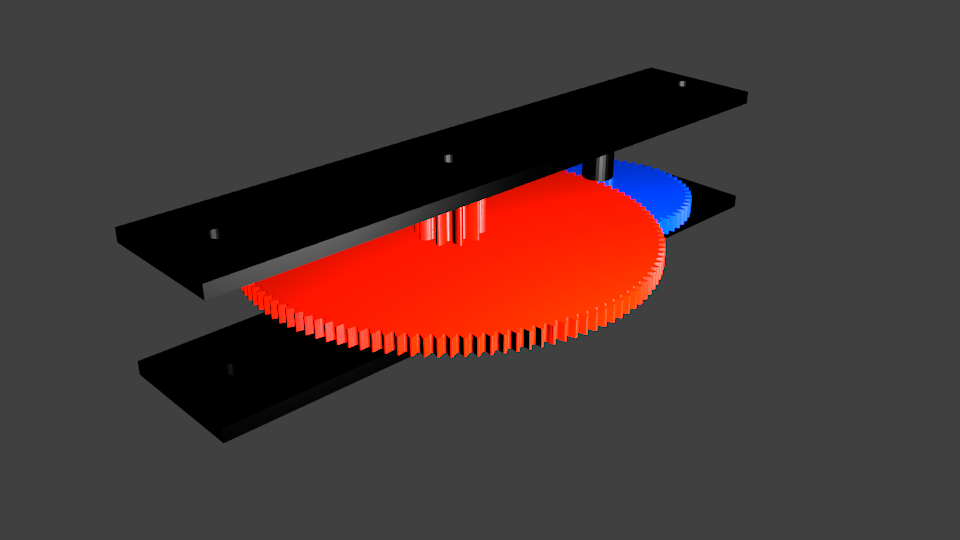
\includegraphics[width=0.45\linewidth]{figures/model2.png}
	\end{tabular}
	
	\caption{Segundo stage propuesto.}
	\label{fig:secondsystem}
\end{figure}

El segundo modelo no fue construido en físico dada la dificultad que se encontró para fabricar las piezas del motoreductor, y su diseño fue reemplazado por el último modelo.

\newpage
\section{Tercer modelo}
Este último fue construido a partir de los planos del Manipulador de BackyardBrains, el cual es de acceso libre, con la posibilidad de realizar modificaciones por los usuarios. Para esto fue necesario la construcción de las piezas del eje $y$ y $z$, dado que las tuercas que se adquirieron eran de dimensiones mucho mayores. Además las bases de los motores fueron diseñadas con el objetivo de obtener un manipulador motorizado. Las piezas fueron diseñadas en Blender, software de uso libre.
\begin{figure}[h]
	\centering
	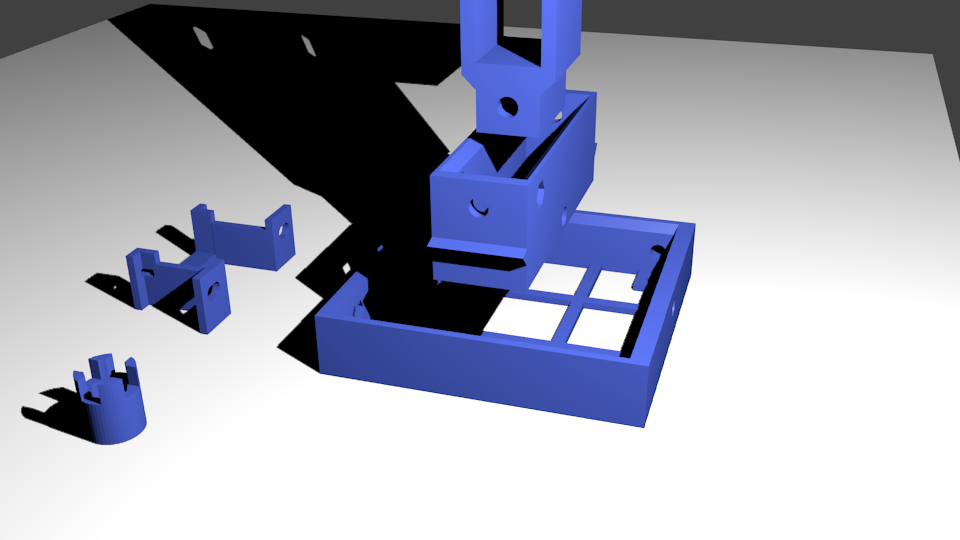
\includegraphics[width=0.9\linewidth]{figures/model3.png}	
	\caption{Tercer stage propuesto.}
	\label{fig:thirdsystem}
\end{figure}

Además de las piezas de impresión, también fue necesario adquirir:
\begin{itemize}
	\item 12 Tornillos M3 de 10 mm.
	\item 2 Tornillos 15/32" de 100 mm.
	\item 1 Tornillo 15/32" de 50 mm.
	\item 12 Tuercas M3.
	\item 6 Tuercas 15/32".
\end{itemize}

Una vez montado el sistema puede moverse las siguientes distancias sobre cada eje, las cuales fueron medidas usando un calibrador Vernier:
\newpage
\begin{table}[h]
	\centering
	\caption{Capacidad en cada dirección del stage.}
	\begin{tabular}{cc}
		\hline
		\textbf{Eje} & \textbf{Distancia (cm)} \\
		\hline
		$x$ & $3.42 \pm 0.01$ \\
		$y$ & $3.90 \pm 0.01$ \\
		$z$ & $1.31 \pm 0.01$ \\
		\hline		
	\end{tabular}
\end{table}

La electrónica es simple, y únicamente fueron necesarios 3 arreglos de transistores Darlington ULN2003, un adaptador de 12 V, y tres motores de paso 28BYJ. El microcontrolador es el mismo usado en el primer modelo, el cual tiene las siguientes tareas: 
\begin{enumerate}
	\item Comunicación con el computador del usuario.
	\item Control de los motores.
\end{enumerate}

El protocolo de comunicación UART establecido envía un mensaje en cada lado de la transmisión de 8 bits, a 4800 baudios. A cada instrucción que envía el computador, el microcontrolador responde \texttt{0xFF} (255 en hexadecimal). Usando el sistema hexadecimal, se usan como primer dígito letras para determinar la identidad del canal, como se muestra en la \autoref{tb:tableUART1}.
\begin{table}[h]
	\centering
	\caption{Identificación de los canales en el protocolo UART.}
	\label{tb:tableUART1}
	\begin{tabular}{cc}
		\hline
		\textbf{Valor} & \textbf{Descripción}\\
		\hline
		A & Canal X \\
		B & Canal Y \\
		C & Canal Z \\
		\hline
	\end{tabular}
\end{table}

Para cada eje es necesario conocer la dirección en la que se desea hacer rotar al motor, la cual es obtenida con el segundo dígito del número hexadecimal.
\begin{table}[h]
	\centering
	\caption{Asignación de la tarea por UART.}
	\label{tb:tableUART2}
	\scriptsize
	\begin{tabular}{cc}
		\hline
		\textbf{Valor} & \textbf{Descripción}\\
		\hline
		0 & Derecha \\
		1 & Izquierda \\
		2 & Pasos: 1 \\
		3 & Pasos: 64 \\
		4 & Pasos: 128 \\
		5 & Pasos: 192 \\
		6 & Pasos: 256 \\
		7 & Pasos: 320 \\
		8 & Pasos: 384 \\
		9 & Pasos: 448 \\
		A & Pasos: 512 \\
		\hline
	\end{tabular}
\end{table}
\newpage

Adicionalmente es posible decirle al microcontrolador que realice varias pasos al motor sin requerir comunicación adicional, es importante decir que el número de pasos para que el motor complete una vuelta es de 512. Con el objetivo de obtener resultados sobre el sistema se realizan mediciones del tiempo requerido para ir y volver hasta el máximo de cada dirección del stage, para varios valores de la resolución (inversos del número de pasos).

En todos los casos se observaron variaciones inferiores al 0.2 \% para resoluciones menores a 9, para el caso de la máxima resolución las variaciones son menores a 1.3 \% en todas las dimensiones, siguiendo la misma forma en todos los casos. Para cada medición se realizaron triplicados, los cuales mostraron desviaciones menores al 0.01\%.

\begin{figure}[h]
	\centering
	\begin{tabular}{cc}
		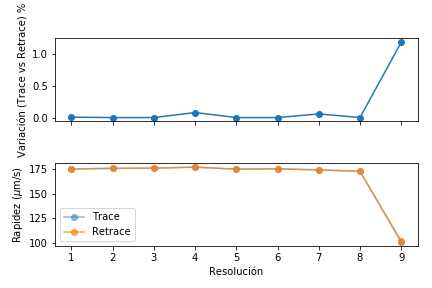
\includegraphics[width=0.5\linewidth]{figures/x.png} & 
		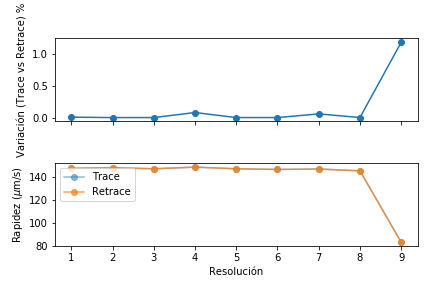
\includegraphics[width=0.5\linewidth]{figures/y.png}
	\end{tabular}
	\caption{Variación y rapidez en función de la resolución para el eje $x$ y $y$, correspondientemente.}
\end{figure}
\begin{figure}[h]
	\centering
	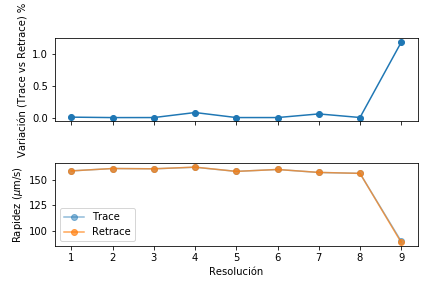
\includegraphics[width=0.45\linewidth]{figures/z.png}
	\caption{Variación y rapidez en función de la resolución para el eje $z$.}
\end{figure}

\newpage
Finalmente y con el objetivo de optimizar el enfoque de un detector sobre una muestra se incluyó en la librería la posibilidad de ingresar 3 puntos $(x, y, z)$ en donde se cumple que la muestra está enfocada, de esta forma es posible obtener un plano que optimiza el enfoque a lo largo de un barrido. Para cada punto del barrido el sistema calcula si debe o no modificarse la altura, por lo que el plano termina en una función de escalones como los que se observan en la \autopageref{fig:plane}, en donde cada cuadro representa las posiciones de medición, el circulo rojo muestra la posición actual del stage.
\begin{figure}[h]
	\centering
	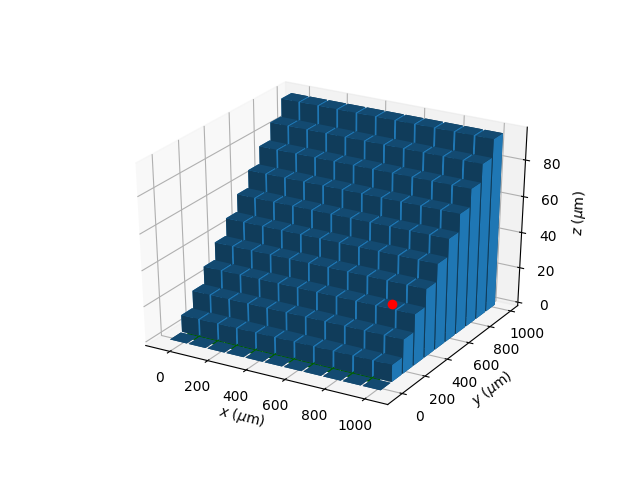
\includegraphics[width=\linewidth]{figures/plane.png}
	\caption{Variación y rapidez en función de la resolución para el eje $z$.}
	\label{fig:plane}
\end{figure}
